\documentclass[../main.tex]{subfiles}
\graphicspath{{\subfix{../images/}}}
\begin{document}

  Para o desenvolvimento do projeto, foi criada uma metodologia própria composta por quatro fases sequenciais, conforme ilustrado na figura \ref{fig:metodologia}. A seguir, será detalhado cada etapa dessa metodologia.

  \begin{figure*}[h]
    \centering
    \caption{Metodologia}
    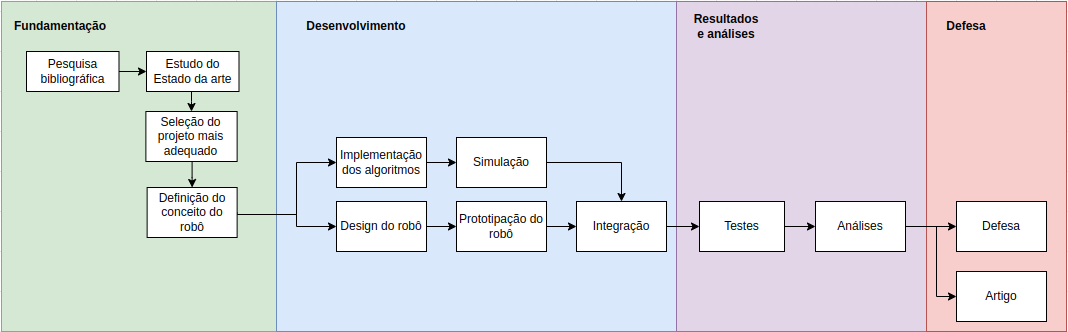
\includegraphics[width=\textwidth]{metodologia.png}

    Fonte: Proprio autor
    \label{fig:metodologia}
  \end{figure*}

  \subsection{Fundamentação}
  A primeira etapa teve como objetivo buscar referências para embasar o estudo os robôs quadrúpedes e servir de padrão para o desenvolvimento do projeto.

  Primeiramente, foi realizada uma pesquisa bibliográfica com o intuito de selecionar artigos relacionados com o projeto. Para realizar essa busca, foi utilizado o método \textit{BILI} (\textit{Bibliographic and Literary Review Method}), que é um método de busca iterativa de artigos, guiada por análises estatísticas das palavras-chave e da rede de co-citação entre os trabalhos encontrados.

  A partir dessa pesquisa, foi possível realizar um estudo do estado da arte com o objetivo de entender a teoria de locomoção dos robôs quadrúpedes. Além disso, foi feito com um \textit{benchmarking} de projetos \textit{open source} desse tipo de sistema robótico, objetivando encontrar referências para a prototipagem. Neste \textit{benchmarking}, foram buscados características que indicassem a viabilidade de prototipação como a disponibilidade do código na internet, linguagem de programação utilizada, disponibilidade do modelo 3D, se foi feito em impressão 3D ou não, tipo dos atuadores, sensores que foram utilizados, entre outras.

  \subsection{Desenvolvimento}
  Durante esta etapa, ocorreu o desenvolvimento do robô propriamente dito. Foram criadas duas frentes de trabalho que ocorreram em paralelo: a implementação e simulação dos algoritmos em ambiente computacional e a criação do \textit{design} junto com a prototipação do robô.

  Durante a implementação dos algoritmos na simulação, foram elaborados, primeiramente, o diagrama de blocos do sistema e a arquitetura de \textit{software} do controlador. A partir disso, os algoritmos de cinemática e controle foram implementados e testados na simulação. Para auxiliar o desenvolvimento do projeto, algumas ferramentas de \textit{softwares} serão utilizadas como o \textit{ROS2 Humble} e o simulador \textit{Gazebo}.

  Em paralelo ao desenvolvimento do \textit{software}, foi realizado o \textit{design} e a prototipação do robô através da elaboração dos desenhos mecânicos e do projeto eletroeletrônico. Esta etapa incluiu também a impressão 3D das partes mecânicas, o teste dos atuadores e sensores e a configuração da comunicação entre a central de processamento e os atuadores, culminando na montagem física do protótipo. Durante essa etapa, o \textit{software} \textit{OnShape} foi utilizado para a modelagem 3D do robô e o \textit{QElectroTech} para o projeto eletroeletrônico.

  Após essas duas etapas, foi possível realizar a integração dos algoritmos no protótipo físico. Ao final da integração, o protótipo já estava funcional e pronto para a fase de testes.

  \subsection{Resultados e análises}
  Durante a etapa de resultados e análises, foram feitos alguns testes para avaliar de forma estatística a performance de locomoção do robô. Também procurou-se avaliar o cumprimento dos requisitos definidos para o protótipo.

  O primeiro experimento realizado consistiu em testar a capacidade do protótipo de mover o pé por uma trajetória cicloidal, feita pelo planejador de trajetórias. Para isso, o corpo do robô foi deixado em um suporte estático, de modo que os pés não tocassem o chão, diminuindo a carga sobre os motores. O objetivo principal deste teste foi verificar se o sistema de controle do robô era capaz de responder de forma coerente aos comandos enviados pelo planejador de marchas numa situação mais próxima da ideal (sem carga). As trajetórias foram calculadas considerando a altura de passo $0,05m$, período de $0,5$ segundos e uma resolução de 25 pontos distribuídos de forma homogênea ($P_T = P_N = 1,0$).
  
  O segundo teste teve como objetivo verificar a capacidade do robô de seguir um comando de velocidade pré-estabelecido e de manter a orientação do seu corpo estável em $0\degree$ nos ângulos de \textit{roll} e \textit{pitch}. O teste foi realizado em dois tipos de terreno: um chão de cimento plano e um terreno irregular formado por pequenas pedras soltas. Este experimento consistiu em enviar um comando de velocidade constante para frente e medir o tempo que o robô precisou para percorrer 1,5 m. Dessa forma, foi possível obter a velocidade média do robô e compará-la com a do comando enviado. Além disso, a fim de avaliar a contribuição do controle de angulação do robô para sua estabilidade, metade dos experimentos foram realizados com esta funcionalidade ativa e a outra não. A estabilidade do robô foi mensurada por meio da oscilação máxima do corpo do robô nos ângulos de \textit{roll} e \textit{pitch}. A trajetória utilizada para o passo possui as mesmas especificações do primeiro experimento, exceto pelos parâmetros de disposição dos pontos, cujos valores adotados foram $P_T = 0,66$ e $P_N = 0,33$. Dessa forma, os testes foram organizados em quatro combinações, variando o tipo do terreno e o uso, ou não, do controle de angulação.
  
  No terceiro experimento, foi avaliada a capacidade do Caramelo de se locomover por terrenos inclinados. Para isso, foi construída uma rampa com uma inclinação de aproximadamente $5,34\degree$ pela qual o robô deveria subir e descer de forma teleoperada. No quarto teste, por fim, foi proposto que o Caramelo atravessasse degraus com diferentes alturas, também de forma teleoperada, a fim de encontrar a máxima altura de obstáculo que ele consegue superar.

\end{document}
